% Options for packages loaded elsewhere
\PassOptionsToPackage{unicode}{hyperref}
\PassOptionsToPackage{hyphens}{url}
%
\documentclass[
]{article}
\usepackage{amsmath,amssymb}
\usepackage{iftex}
\ifPDFTeX
  \usepackage[T1]{fontenc}
  \usepackage[utf8]{inputenc}
  \usepackage{textcomp} % provide euro and other symbols
\else % if luatex or xetex
  \usepackage{unicode-math} % this also loads fontspec
  \defaultfontfeatures{Scale=MatchLowercase}
  \defaultfontfeatures[\rmfamily]{Ligatures=TeX,Scale=1}
\fi
\usepackage{lmodern}
\ifPDFTeX\else
  % xetex/luatex font selection
\fi
% Use upquote if available, for straight quotes in verbatim environments
\IfFileExists{upquote.sty}{\usepackage{upquote}}{}
\IfFileExists{microtype.sty}{% use microtype if available
  \usepackage[]{microtype}
  \UseMicrotypeSet[protrusion]{basicmath} % disable protrusion for tt fonts
}{}
\makeatletter
\@ifundefined{KOMAClassName}{% if non-KOMA class
  \IfFileExists{parskip.sty}{%
    \usepackage{parskip}
  }{% else
    \setlength{\parindent}{0pt}
    \setlength{\parskip}{6pt plus 2pt minus 1pt}}
}{% if KOMA class
  \KOMAoptions{parskip=half}}
\makeatother
\usepackage{xcolor}
\usepackage[margin=1in]{geometry}
\usepackage{color}
\usepackage{fancyvrb}
\newcommand{\VerbBar}{|}
\newcommand{\VERB}{\Verb[commandchars=\\\{\}]}
\DefineVerbatimEnvironment{Highlighting}{Verbatim}{commandchars=\\\{\}}
% Add ',fontsize=\small' for more characters per line
\usepackage{framed}
\definecolor{shadecolor}{RGB}{248,248,248}
\newenvironment{Shaded}{\begin{snugshade}}{\end{snugshade}}
\newcommand{\AlertTok}[1]{\textcolor[rgb]{0.94,0.16,0.16}{#1}}
\newcommand{\AnnotationTok}[1]{\textcolor[rgb]{0.56,0.35,0.01}{\textbf{\textit{#1}}}}
\newcommand{\AttributeTok}[1]{\textcolor[rgb]{0.13,0.29,0.53}{#1}}
\newcommand{\BaseNTok}[1]{\textcolor[rgb]{0.00,0.00,0.81}{#1}}
\newcommand{\BuiltInTok}[1]{#1}
\newcommand{\CharTok}[1]{\textcolor[rgb]{0.31,0.60,0.02}{#1}}
\newcommand{\CommentTok}[1]{\textcolor[rgb]{0.56,0.35,0.01}{\textit{#1}}}
\newcommand{\CommentVarTok}[1]{\textcolor[rgb]{0.56,0.35,0.01}{\textbf{\textit{#1}}}}
\newcommand{\ConstantTok}[1]{\textcolor[rgb]{0.56,0.35,0.01}{#1}}
\newcommand{\ControlFlowTok}[1]{\textcolor[rgb]{0.13,0.29,0.53}{\textbf{#1}}}
\newcommand{\DataTypeTok}[1]{\textcolor[rgb]{0.13,0.29,0.53}{#1}}
\newcommand{\DecValTok}[1]{\textcolor[rgb]{0.00,0.00,0.81}{#1}}
\newcommand{\DocumentationTok}[1]{\textcolor[rgb]{0.56,0.35,0.01}{\textbf{\textit{#1}}}}
\newcommand{\ErrorTok}[1]{\textcolor[rgb]{0.64,0.00,0.00}{\textbf{#1}}}
\newcommand{\ExtensionTok}[1]{#1}
\newcommand{\FloatTok}[1]{\textcolor[rgb]{0.00,0.00,0.81}{#1}}
\newcommand{\FunctionTok}[1]{\textcolor[rgb]{0.13,0.29,0.53}{\textbf{#1}}}
\newcommand{\ImportTok}[1]{#1}
\newcommand{\InformationTok}[1]{\textcolor[rgb]{0.56,0.35,0.01}{\textbf{\textit{#1}}}}
\newcommand{\KeywordTok}[1]{\textcolor[rgb]{0.13,0.29,0.53}{\textbf{#1}}}
\newcommand{\NormalTok}[1]{#1}
\newcommand{\OperatorTok}[1]{\textcolor[rgb]{0.81,0.36,0.00}{\textbf{#1}}}
\newcommand{\OtherTok}[1]{\textcolor[rgb]{0.56,0.35,0.01}{#1}}
\newcommand{\PreprocessorTok}[1]{\textcolor[rgb]{0.56,0.35,0.01}{\textit{#1}}}
\newcommand{\RegionMarkerTok}[1]{#1}
\newcommand{\SpecialCharTok}[1]{\textcolor[rgb]{0.81,0.36,0.00}{\textbf{#1}}}
\newcommand{\SpecialStringTok}[1]{\textcolor[rgb]{0.31,0.60,0.02}{#1}}
\newcommand{\StringTok}[1]{\textcolor[rgb]{0.31,0.60,0.02}{#1}}
\newcommand{\VariableTok}[1]{\textcolor[rgb]{0.00,0.00,0.00}{#1}}
\newcommand{\VerbatimStringTok}[1]{\textcolor[rgb]{0.31,0.60,0.02}{#1}}
\newcommand{\WarningTok}[1]{\textcolor[rgb]{0.56,0.35,0.01}{\textbf{\textit{#1}}}}
\usepackage{graphicx}
\makeatletter
\def\maxwidth{\ifdim\Gin@nat@width>\linewidth\linewidth\else\Gin@nat@width\fi}
\def\maxheight{\ifdim\Gin@nat@height>\textheight\textheight\else\Gin@nat@height\fi}
\makeatother
% Scale images if necessary, so that they will not overflow the page
% margins by default, and it is still possible to overwrite the defaults
% using explicit options in \includegraphics[width, height, ...]{}
\setkeys{Gin}{width=\maxwidth,height=\maxheight,keepaspectratio}
% Set default figure placement to htbp
\makeatletter
\def\fps@figure{htbp}
\makeatother
\setlength{\emergencystretch}{3em} % prevent overfull lines
\providecommand{\tightlist}{%
  \setlength{\itemsep}{0pt}\setlength{\parskip}{0pt}}
\setcounter{secnumdepth}{-\maxdimen} % remove section numbering
\ifLuaTeX
  \usepackage{selnolig}  % disable illegal ligatures
\fi
\usepackage{bookmark}
\IfFileExists{xurl.sty}{\usepackage{xurl}}{} % add URL line breaks if available
\urlstyle{same}
\hypersetup{
  pdftitle={M9 Problem Set: One Way ANOVA for TAs},
  pdfauthor={Pablo E. Gutierrez-Fonseca},
  hidelinks,
  pdfcreator={LaTeX via pandoc}}

\title{M9 Problem Set: One Way ANOVA for TAs}
\author{Pablo E. Gutierrez-Fonseca}
\date{2024-05-06 14:31:10}

\begin{document}
\maketitle

Consider an example in which a researcher is investigating the
\textbf{impact of metal contamination on the diversity of species found
in sessile marine invertebrates such as sponges, bryozoans, and sea
squirts}. The researcher aims to determine whether \textbf{copper
reduces species richness}, while \textbf{also considering the potential
influence of substrate orientation, whether vertical or horizontal}, on
invertebrate richness.

To address this, they conducted an experiment where species richness was
assessed in replicate samples under each of the six combinations of
copper enrichment levels (\textbf{``None,'' ``Low,'' ``High''}) and
substrate orientations (\textbf{``Vertical,'' ``Horizontal''}). This
experimental design is referred to as factorial, as it encompasses all
levels of one treatment within all levels of the other treatment, also
known as orthogonal.

\textbf{The factorial ANOVA will test the following hypotheses:}\\
1. Whether there are differences in richness among the three levels of
copper enrichment.\\
2. Whether there are differences in richness among the two levels of
substrate orientation.\\
3. Whether there is an interaction effect between copper enrichment and
substrate orientation, indicating whether the effect of copper on
richness depends on the orientation of the substrate.

Summarize: Write a concise one paragraph summary of this analysis.
Remember that any summary should include the following:\\
1. Statement of the research hypothesis or study objectives.\\
2. Brief summary of methods (one sentence or less).\\
3. Statement of the statistical results (including type of test and
shorthand: F(df)= obtained value, p = 0.xxx). Include results of the
possible interaction between copper enrichment and substrate
orientation.\\
4. Description of any differences, if meaningful, along with an
interpretation of why these results make sense (or don't make sense).

\#1. Import libraries and load packages

\begin{Shaded}
\begin{Highlighting}[]
\FunctionTok{library}\NormalTok{(tidyverse)}
\end{Highlighting}
\end{Shaded}

\begin{verbatim}
## Warning: package 'tidyverse' was built under R version 4.3.2
\end{verbatim}

\begin{verbatim}
## Warning: package 'ggplot2' was built under R version 4.3.3
\end{verbatim}

\begin{verbatim}
## Warning: package 'tibble' was built under R version 4.3.1
\end{verbatim}

\begin{verbatim}
## Warning: package 'tidyr' was built under R version 4.3.2
\end{verbatim}

\begin{verbatim}
## Warning: package 'readr' was built under R version 4.3.2
\end{verbatim}

\begin{verbatim}
## Warning: package 'purrr' was built under R version 4.3.1
\end{verbatim}

\begin{verbatim}
## Warning: package 'dplyr' was built under R version 4.3.2
\end{verbatim}

\begin{verbatim}
## Warning: package 'stringr' was built under R version 4.3.2
\end{verbatim}

\begin{verbatim}
## Warning: package 'forcats' was built under R version 4.3.2
\end{verbatim}

\begin{verbatim}
## Warning: package 'lubridate' was built under R version 4.3.2
\end{verbatim}

\begin{Shaded}
\begin{Highlighting}[]
\FunctionTok{library}\NormalTok{(lessR)}
\end{Highlighting}
\end{Shaded}

\begin{verbatim}
## Warning: package 'lessR' was built under R version 4.3.2
\end{verbatim}

\begin{Shaded}
\begin{Highlighting}[]
\FunctionTok{library}\NormalTok{(readxl)}
\FunctionTok{library}\NormalTok{(dplyr)}
\end{Highlighting}
\end{Shaded}

\begin{Shaded}
\begin{Highlighting}[]
\NormalTok{Sessile }\OtherTok{\textless{}{-}} \FunctionTok{read.csv}\NormalTok{(}\AttributeTok{file =} \StringTok{"Sessile.csv"}\NormalTok{, }\AttributeTok{header =} \ConstantTok{TRUE}\NormalTok{)}
\end{Highlighting}
\end{Shaded}

\begin{Shaded}
\begin{Highlighting}[]
\NormalTok{Sessile.aov }\OtherTok{\textless{}{-}} \FunctionTok{aov}\NormalTok{(Richness }\SpecialCharTok{\textasciitilde{}}\NormalTok{ Copper }\SpecialCharTok{*}\NormalTok{ Orientation, }\AttributeTok{data =}\NormalTok{ Sessile)}
\FunctionTok{summary}\NormalTok{(Sessile.aov)}
\end{Highlighting}
\end{Shaded}

\begin{verbatim}
##                    Df Sum Sq Mean Sq F value               Pr(>F)    
## Copper              2   3330  1665.0  192.53 < 0.0000000000000002 ***
## Orientation         1    240   240.0   27.75       0.000002463599 ***
## Copper:Orientation  2    571   285.3   33.00       0.000000000434 ***
## Residuals          54    467     8.6                                 
## ---
## Signif. codes:  0 '***' 0.001 '**' 0.01 '*' 0.05 '.' 0.1 ' ' 1
\end{verbatim}

\begin{Shaded}
\begin{Highlighting}[]
\FunctionTok{interaction.plot}\NormalTok{(Sessile}\SpecialCharTok{$}\NormalTok{Copper, Sessile}\SpecialCharTok{$}\NormalTok{Orientation, Sessile}\SpecialCharTok{$}\NormalTok{Richness)}
\end{Highlighting}
\end{Shaded}

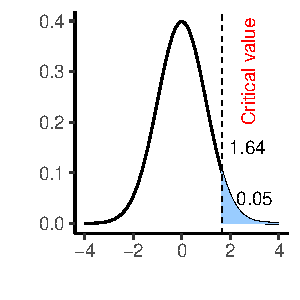
\includegraphics{M10-Problem-Set-Factorial-ANOVA-TAs_files/figure-latex/unnamed-chunk-4-1.pdf}

References:
\url{https://environmentalcomputing.net/statistics/linear-models/anova/anova-factorial/}

\end{document}
